\documentclass{article}
\usepackage[spanish]{babel}
% \usepackage{lipsum}
% \usepackage{natbib}
% \usepackage{graphicx}
\usepackage{analysis_orax}
\usepackage{changepage}
\usepackage{enumitem}% \setlist

\usepackage[colorlinks=true,urlcolor=blue,linkcolor=black,anchorcolor=blue]{hyperref}

\usepackage[defaultlines=10,all]{nowidow}

\providecommand{\tightlist}{%
          \setlength{\itemsep}{0pt}\setlength{\parskip}{0pt}}
          
\newcommand{\headerline}[3]{%
  \par\medskip\noindent
  \makebox[0pt][l]{#1}%
  \makebox[20.5cm][c]{\textbf{#2}}%
  \makebox[0pt][r]{#3}\par\medskip}

\definecolor{bannergray}{HTML}{2E2F34}
\definecolor{bannerred}{HTML}{F07468}
\definecolor{bannertec}{HTML}{00447B}




%------------------Document----------------------------

\begin{document}

%-------------------------TitlePage------------------------
%\begin{titlepage}
%\end{titlepage}

\begingroup
\thispagestyle{empty}
\begin{tikzpicture}[remember picture,overlay]

\coordinate [below=5.15cm,left=-5cm] (midpoint) at (current page.north);
\coordinate [below=29.2cm,left=-5cm] (downpoint) at (current page.north);

\node at (current page.north west)
{\begin{tikzpicture}[remember picture,overlay]
\node[anchor=north west,inner sep=0pt] at (0,-2.3) {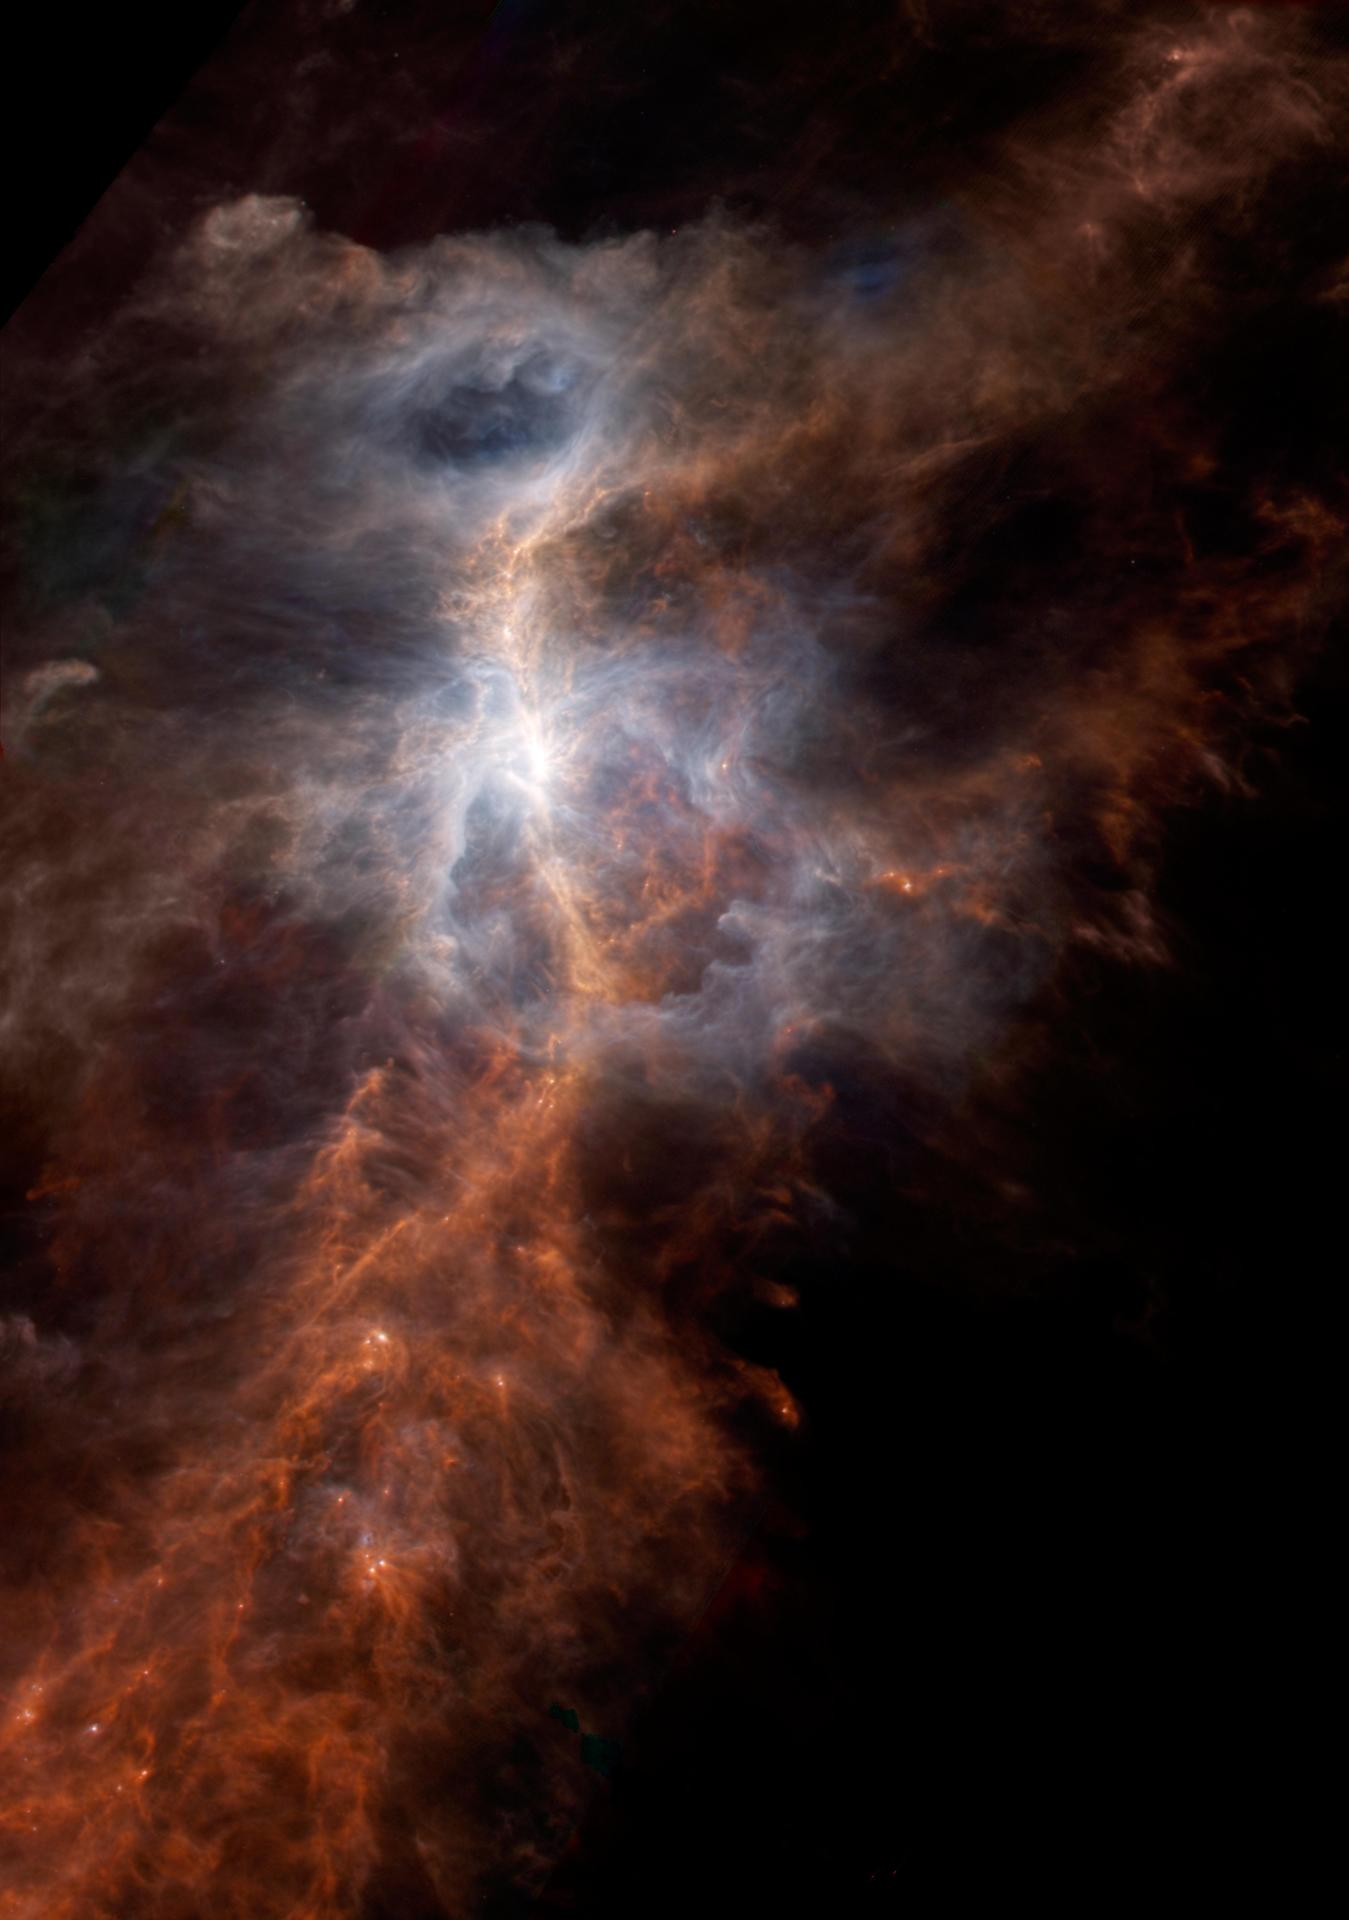
\includegraphics[width=\paperwidth,height=30cm]{figures/PIA21073large.jpg}}; % Background image

\node[anchor=north west,inner sep=0pt] at (1,-0.5cm) {
\includegraphics[scale=0.4]{figures/logo_tec.png}}; % logotec

\draw[anchor=north] (midpoint) node [fill=bannergray,fill opacity=0.8,text opacity=1,inner sep=1cm]{

	\Huge\bfseries\sffamily\parbox[c][][t]{\paperwidth}{
			\centering \Large \color{white} Proyecto 1 \\[5pt] % Book title
			{\Huge \color{bannerred} QR-Net	}\\[20pt] % Subtitle
			{\small Junio, 2019}
		}

}; % Proyect Name

\draw[anchor=north] (downpoint) node [fill=bannertec,fill opacity=1,text opacity=1,inner sep=0.5cm]{

	\color{white}\normalsize\sffamily\parbox[c][][t]{\paperwidth}{
%			\centering \color{white} Ingenieria en Computacion - Redes - Prof. Kevin Moraga
			\headerline{Ingenieria en Computacion}{Redes de Computadoras}{Prof. Kevin Moraga}
		}

}; % Author


\end{tikzpicture}};
\end{tikzpicture}
\vfill
\endgroup

\newpage

\begin{tikzpicture}[remember picture,overlay]

\coordinate [below=10.15cm,left=2.8cm] (objectivopoint) at (current page.north);
\coordinate [below=10.5cm,left=2.8cm] (datosgeneralespoint) at (current page.north);

\draw[anchor=south] (objectivopoint) node [fill=bannertec,fill opacity=0.8,text opacity=1,inner sep=1cm]{

	\color{white}\sffamily\parbox[c][6cm][t]{6cm}{
			\vfill
			{\bfseries \huge  Objetivo} \\[5pt] % Book title
			\large Realizar una re-implementación de algunas de las funciones de varias capas del modelo OSI. Incluyendo la creación de un RFC
		}

}; % Objetivo

\draw[anchor=north] (datosgeneralespoint) node [fill=bannergray,fill opacity=0.8,text opacity=1,inner sep=1cm]{

	\color{white}\sffamily\parbox[c][11.5cm][t]{6cm}{
			{\bfseries \huge  Datos Generales} \\[5pt] % Book title
			\large 
			\begin{itemize}
				\item \textbf{Fecha de Entrega:} \\ Jueves 09 de Mayo de 2019 antes de las 23:59:59 GMT-6.
				\item \textbf{Fecha de Revision:} \\ Viernes 10 de Mayo de 2019	
				\item \textbf{Lenguaje:} \\ Java, C o python para GNU/Linux
				\item \textbf{Recurso Humano:}\\ Grupos de 3
				\item \textbf{Valor de la asignacion:} 10\%				
			\end{itemize}			
			\vspace{1cm}
			{\bfseries \huge  Profesor} \\[5pt] % Book title
			Kevin Moraga\\
			kmoraga@ic-itcr.ac.cr\\
			Ingenieria en Computacion
			
		}

}; % Objetivo



\end{tikzpicture}



\begin{adjustwidth}{8.8cm}{}
~\vfill

%-------------------------Content------------------------
\section{Introducción}\label{introducciuxf3n}
\large
\begin{sloppypar}
Actualmente el tema de anonimato se encuentra cada vez más en el plano
principal de discusión en el mundo. Esto debido a que en el pasado,
pueblos han sufrido y su historia se ha visto manchada. Debido a ello se
han promulgado acuerdos internacionales en pro de los derechos humanos.
Y uno en especial (Artículo 19) de la libertad de expresión.

A pesar que hoy 2019 nos encontramos en un momento privilegiado en la
historia, hay países donde aún se siguen teniendo problemas de libertad
de expresión. Desde el poder comunicarse debido aque las TELCOS locales
no les interesa invertir en pueblos donde tiene pérdidas, lugares donde
el gobierno calla a sus habitantes y hasta lugares donde la privacidad
es una cuestión de vida o muerte.

Por lo anterior, el objetivo del proyecto es conocer distintas
soluciones que nos permitan acercarnos más a esa libertad de expresión
sin excepciones.
\end{sloppypar}

\vspace{2cm}

\end{adjustwidth}


\newcommand{\sectionbreak}{\clearpage}

\section{Requerimientos Funcionales}\label{requerimientos-funcionales}

\subsection{Capa 1: Medio Físico}\label{capa-1-medio-fuxedsico}

\begin{itemize}
\tightlist
\item
  El medio físico a utilizar será luz con códigos QR.
\item
  Esta capa será administrada por un dispositivo con cámara, por lo que
  este dispositivo funcionará como una interfaz de red. Ahora en
  adelante lo llamaremos ``Dispositivo de Transmisión''.
\item
  Esta interfaz de red se comunicará con una computadora común de
  escritorio a través de un protocolo definido por el estudiante. Lo que
  permitiría a dos nodos enviar paquetes a través del ``Dispositivo de
  Transmisión''
\item
  Es necesario implementar un protocolo de comunicación que gobierne la
  interacción de los paquetes, generando una trama con un tamaño máximo
  de 128 bytes.
\item
  El diseño de esta trama queda en manos del estudiante, este diseño
  debe de cumplir con las restricciones del presente enunciado.
\item
  Debe existir una biblioteca llamada ``DispositivoLuzAdaptador'' que se
  encargue de la comunicación entre el nodo y el ``Dispositivo de
  Transmisión''.
\item
  Algunas restricciones para el diseño:

  \begin{itemize}
  \tightlist
  \item
    Tamaño máximo de la trama 128 bytes
  \item
    Debe de realizar la verificación de checksum.
  \item
    Debe de proveer un manejo de Acceso al medio.
  \item
    Debe incluir manejo de versiones del protocolo.
  \item
    Se debe de crear una dirección física (un análogo al MAC Address),
    que permita conectar múltiples equipos a la misma red.
  \end{itemize}
\end{itemize}

\subsection{Capa 2 y 3: QR-Net}\label{capa-2-y-3-qr-net}

QR-Net es una red que funciona sobre cualquier red TCP/IP. Esta red
consiste en una red mesh, la cual se encarga de pasar paquetes de forma
anónima. O sea, se debe de implementar algún mecanismo en el protocolo
el cual permita la comunicación a través de la red mesh, sin que esta
red revele la persona que lo originó.

Además en QR-Net existen distintas ciudades, estas están separadas por
muchos kilómetros de distancia. Y por ello se tiene al menos un par de
puertas de enlace que permita la comunicación entre las dos ciudades
utilizando el ``Dispositivo de Transmisión''.

A través de la red de QR-Net, se deberán de rutear los paquetes a través
de los distintos dispositivo que se encuentren asociados. Cada
dispositivo deberá de poder transmitir al siguiente dispositivo que esté
más cerca del destino. Se recomienda el uso de circuitos virtuales,
previamente negociados.

Los canales a utilizar son:

\begin{itemize}
\tightlist
\item
  Ethernet
\item
  Wifi 802.11x
\item
  Dispositivo de Transmisión
\item
  VPN
\end{itemize}

En resumen, es necesario tener un control de lo siguiente:

\begin{itemize}
\tightlist
\item
  Enrutamiento negociado: Se realizará enrutamiento dinámico a través de
  la red mesh.
\item
  Directorio de nodos: Es un servicio donde se comparten los nodos
  entrantes a QR-Net
\end{itemize}

\subsection{Capa 4: Aplicación
(QR-Net)}\label{capa-4-aplicaciuxf3n-qr-net}

El principal objetivo de QR-Net es ser una red de microblogging o bien
que permita el chat entre personas. Por lo que el microblogging o chat
reside únicamente en QR-Net

\subsection{Capa 4: Aplicación
(clearnet)}\label{capa-4-aplicaciuxf3n-clearnet}

Para la capa de aplicación se deberá realizar la instalación de un
servidor IRC conocido. En este servidor debe de correr un bot que se
encargue de realizar la comunicación con QR-Net. Solo los chat
etiquetados como públicos deben de salir a clearnet.

Además cada vez que existe una entrada de un tópico en particular debe
de publicar que hay una nueva entrada en un servidor de nntp.

\subsection{RFC}\label{rfc}

La documentación del diseño incluye la creación de un RFC, esto
incluyendo las normas estándar que rigen los RFC. Todo el RFC debe de
estar en ASCII, incluyendo los diagramas. Se pude basar en el RFC 2616
de HTTP. Este se puede encontrar en el siguiente
\href{http://www.w3.org/Protocols/rfc2616/rfc2616.txt}{enlace}

\subsection{Otras consideraciones}\label{otras-consideraciones}

Además de las definiciones anteriores tome en cuenta:

\begin{itemize}
\tightlist
\item
  Debe crear el RFC para el protocolo de QR-Net.
\item
  Puede utilizar la biblioteca Scapy.
\item
  El diseño de la Capa 1, debería ser lo suficientemente versátil para
  permitir datacasting de archivos grandes, a través del código QR.
\item
  Todos los protocolos deben tener una forma de cambiar la versión,
  anticipándose a futuros releases del protocolo, con nuevas
  definiciones.
\item
  El tamaño de campos dinámicos de una trama o paquete deben de estar
  definidos en un campo por aparte.
\end{itemize}

\subsection{Extra}\label{extra}

El grupo que pueda alcanzar la mayor tasa de transferencia de datos, en
el datacasting de QR, tendrá un puntaje adicional. Este puntaje quedará
a criterio del profesor. Y se podrá también ditribuir puntaje adicional
para grupos adicionales.

\section{Cuestiones administrativas}\label{administrativo}

\subsection{Entregables}\label{entregables}

\begin{itemize}
\tightlist
\item
  Código fuente del programa que cumpla los requerimientos funcionales y
  técnicos.
\item
  Binario del programa, compilado para una arquitectura x86.
\item
  Fuente de la documentación en Markdown o en Latex y luego a PDF.
\item
  PDF con la documentación.
\end{itemize}

\subsection{Evaluación}\label{evaluaciuxf3n}

\begin{itemize}
\tightlist
\item
  Capa 1 - Dispositivo de Tranmsisión: 20\%
\item
  QR-Net: 30\%
\item
  Capa 4 - Aplicación (QR-Net): 10\%
\item
  Capa 4 - Aplicación (clearnet): 10\%
\item
  RFC: 10\%
\item
  Documentación: 20\%
\item
  Extra: 10\%
\end{itemize}

\subsection{Documentación}\label{documentaciuxf3n}

Las siguientes son las instrucciones para la documentación. NO LA
IMPRIMA. Además la documentación se debe de realizar utilizando MD con
Latex.

\begin{enumerate}
\def\labelenumi{\arabic{enumi}.}
\tightlist
\item
  \textbf{Introducción}: Presentar el problema. Puede ``reciclar''
  partes del enunciado de la tarea programada.
\item
  \textbf{Ambiente de desarrollo}: Indicar las herramientas usadas para
  implementar la tarea.
\item
  \textbf{Estructuras de datos usadas y funciones}: Se debe describir
  las principales funciones y estructuras utilizadas en la elaboración
  de esta asignación.
\item
  \textbf{Instrucciones para ejecutar el programa}: Presentar las
  consultas concretas usadas para correr el programa para el problema
  planteado en el enunciado de la tarea y para los casos planteados al
  final de esta documentación.
\item
  \textbf{Actividades realizadas por estudiante}: Este es un resumen de
  las bitácoras de cada estudiante ( estilo timesheet) en términos del
  tiempo invertido para una actividad específica que impactó
  directamente el desarrollo del trabajo, de manera breve (no más de una
  línea) se describe lo que se realizó, la cantidad de horas invertidas
  y la fecha en la que se realizó. Se deben sumar las horas invertidas
  por cada estudiante, sean conscientes a la hora de realizar esto el
  profesor determinará si los reportes están acordes al producto
  entregado.
\item
  \textbf{Comentarios finales (estado del programa)}: Indicar el estado
  final en que quedó el programa, problemas encontrados y limitaciones
  adicionales.
\item
  \textbf{Conclusiones} y Recomendaciones del proyecto.
\item
  \textbf{Bibliografía} utilizada en la elaboración de la presente
  asignación.
\item
  Es necesario documentar el código fuente.
\end{enumerate}

\subsection{Aspectos Adicionales}\label{aspectos-adicionales}

Aún cuando el código y la documentación tienen sus notas por separado,
se aplican las siguientes restricciones:

\begin{enumerate}
\def\labelenumi{\arabic{enumi}.}
\tightlist
\item
  Sí no se entrega documentación, automáticamente se obtiene una nota de
  0.
\item
  Sí el código no compila se obtendrá una nota de 0, por lo cuál se
  recomienda realizar la defensa con un código funcional.
\item
  El código debe ser desarrollado en el lenguaje especificado en los
  Datos Generales, en caso contrario se obtendrá una nota de 0.
\item
  Sí no se siguen las reglas del formato del envío a través de Google
  Drive se obtendrá una nota de 0.
\item
  La revisión de la documentación será realizada por parte del profesor,
  no durante la defensa del proyecto.
\item
  Cada grupo tendrá como máximo 20 minutos para exponer su trabajo al
  profesor y realizar la defensa de éste, es responsabilidad de los
  estudiantes mostrar todo el trabajo realizado, por lo cuál se
  recomienda tener todo listo antes de ingresar a la defensa.
\item
  Cada excepción o error que salga durante la ejecución del proyecto y
  que se considere debió haber sido contemplada durante el desarrollo
  del proyecto, se castigará con 2 puntos de la nota final de la
  presente asignación.
\item
  Cada grupo es responsable de llevar los equipos requeridos para la
  revisión, si no cuentan con estos deberá avisar al menos 2 días antes
  de la revisión al profesor para coordinar el préstamo de estos.
\item
  Durante la revisión podrán participar asistentes, otros profesores y
  el coordinador del área.
\item
  Cualquier indicio de copia será calificado con una nota de 0 y será
  procesado de acuerdo al reglamento.
\end{enumerate}

~\vfill

% %-------------------------Content------------------------


\end{document}
